\documentclass[11pt]{article}
\usepackage{../EllioStyle}

\title{Homework 2}
\author{Elliott Pryor \\
Collaborated with: Nathan Stouffer}
\date{11 Feb 2021}

\rhead{Homework 2}
\lhead{Elliott Pryor}

\graphicspath{{./}{images/}}




\makeatletter
\def\mathcolor#1#{\@mathcolor{#1}}
\def\@mathcolor#1#2#3{%
  \protect\leavevmode
  \begingroup
    \color#1{#2}#3%
  \endgroup
}
\makeatother


\algdef{SE}[DOWHILE]{Do}{doWhile}{\algorithmicdo}[1]{\algorithmicwhile\ #1}

\begin{document}
\maketitle

\problem{1}

Assume you are given a planar subdivision with $n$ faces in a DCEL. (You may
assume that the planar subdivision does not contain any holes, i.e., there are
no nested faces.) Give pseudo-code for an algorithms that given a vertex $v$ of
the DCEL, outputs all neighbors of $v$.

\hrule

\begin{algorithm}
    \caption{Find Neighbors}
    \label{alg:neighbors}
    \begin{algorithmic}[1]
    \Function{Neighbors}{$v$}
        \State $start \gets v.incident\_edge$
        \State $e \gets start$
        \Do
            \State $twin \gets e.twin$
            \State add $twin.origin$ to neighbors
            \State $e \gets twin.next$
        \doWhile{$e \neq start$}
        \State \textbf{return} neighbors
    \EndFunction
    \end{algorithmic}
\end{algorithm}


\begin{figure}[h]
    \centering
    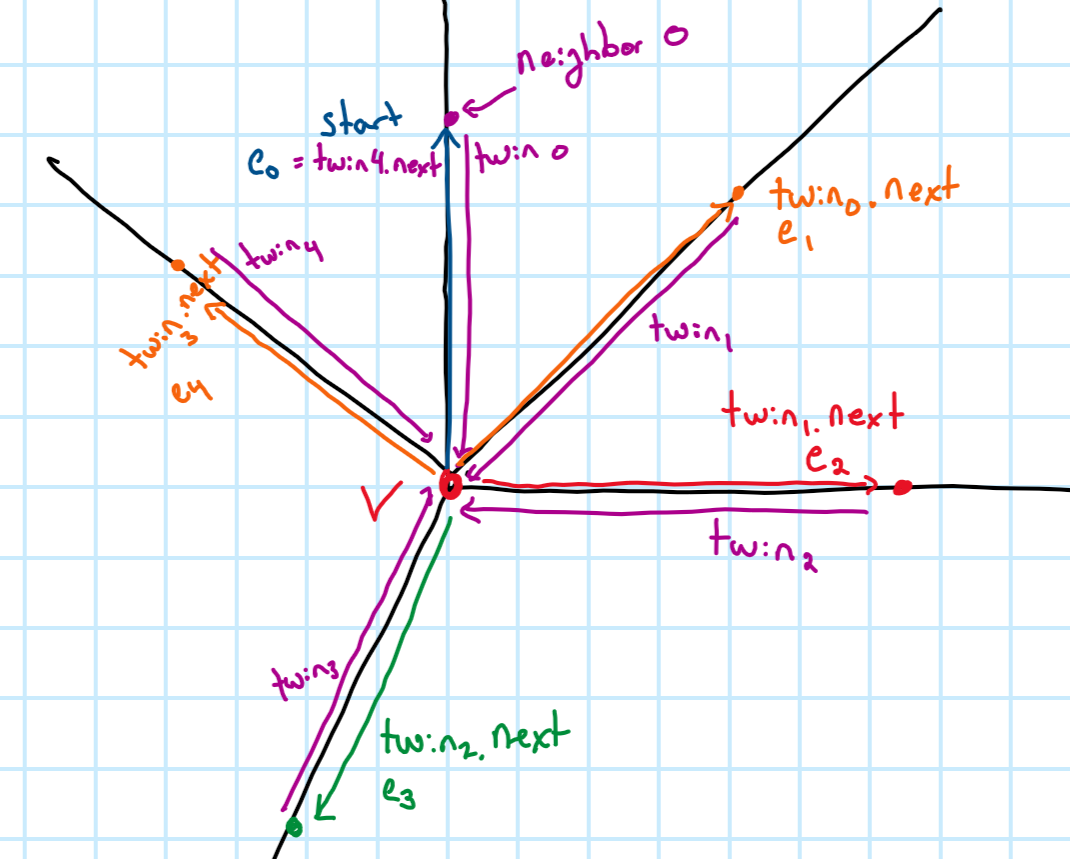
\includegraphics[width = 0.65\textwidth]{prob1}
    \caption{Problem 1: Visual demonstration of algorithm}
\end{figure}

\textbf{Correctness:} The algorithm starts with the incident edge to vertex $v$. 
Since we only store the origin of each edge, the origin of the twin is the same as the destination.
This is a neighbor of $v$ since it is 1 edge away. 
Then, we observe that if $e$ is incident on the left face, then $e.twin$ is incident on the right face.

We also know that the destination of $e.twin$ is $v$. So $e.twin.next$ must be another neighbor of $v$.
This is the next neighbor clockwise around $v$. Suppose we skipped a neighbor then there must be a face in between.
But then twin would have to be incident on the middle face (one in between), so a contradiction and we find the next node clockwise.

So we always find the next neighbor clockwise around $v$, until we reach the start when we terminate.

\textbf{Running Time:} We cover each face that $v$ is incident upon once. Therefore our time is $O(n)$




\problem{2}

Assume you are given a planar subdivision of $O(n)$ size in a DCEL. (You may
assume that the planar subdivision does not contain any holes, i.e., there are
no nested faces.) Describe an algorithm that for a given point $p$ in the plane
finds the face in the subdivision that contains it. Your algorithm should run in
$O(n)$ time. You do not have to write pseudo-code, but please make clear what
DCEL operations you are using. Also please make sure the analysis is detailed
enough to justify the $O(n)$ runtime clearly.

\hrule


We start by drawing a ray in the +x direction originating at $p$.
We then pick any face and walk around all the edges. We count the number of times
the ray intersects any edge. If this is even, then the point is not inside, otherwise it is inside.
Note this only works if we assume that the point $p$ is not in any region unbounded along the $x$ axis.
If this is the case, we can add an imaginary edge very far away. 

We then do this for all the faces until we find one that it is in.

\begin{algorithm}
    \caption{Find what face Point is in}
    \label{alg:point}
    \begin{algorithmic}[1]
    \Function{FindFace}{$p$}
        \For{face $\in$ Faces}
            \State $start \gets face.incident\_edge$
            \State $e \gets start$
            \State $intersections \gets 0$
            \Do
                \State $origin \gets e.origin$, $destination \gets e.twin.origin$
                \State $l \gets$ line through edge $e$
                \State $i \gets $ point where $l(x) = p_y$ \textcolor{red}{point where line interesects y level of p}
                \If{$i.x \geq p.x$ and $i.x \in [origin.x, destination.x]$}
                    \State \textcolor{red}{Found an intersection!}
                    \State increment $intersections$
                \EndIf
                \State $e \gets e.next$
            \doWhile{$e \neq start$}
            \If {$intersections$ is odd}
                \State \textbf{return} face
            \EndIf
        \EndFor
    \EndFunction
    \end{algorithmic}
\end{algorithm}


\textbf{Correctness: } We first show that a point is inside a polygon if and only if a ray in the +x direction 
intersects the edges an odd number of times. 

\begin{proof}
    
    Let $r$ be a ray in the $+x$ direction originating at $p$. Let $P$ be a bounded polygon. 
    Crossing $P$ refers to crossing the boundary of $P$, and $\in P$ refers to inside the region bounded by $P$.

    Forward Direction: Assume that $p$ is inside $P$ then we show that it interesects an odd number of times.
    Since, $p \in P$ then certainly the ray crosses the boundary of $P$ at least once. Then if $r$ enters $P$,
    it certainly had to of first left it. So there is a parity. It must cross once to leave, and once to return (2).
    But since it is bounded, it will eventually cross to leave without entering. Thus the number of intersections is odd.

    Reverse Direction: Assume that the number of times $r$ crosses $P$ an odd number of times, then we show $p \in P$.
    Since the number of intersections is odd, then the ray either entered $P$ and never left,
    or left $P$ without first entering. The first case is impossible since $P$ is bounded. 
    Then, the only way for the second case to occur is if $p \in P$
\end{proof}

Thus we can correctly determine if the point is inside a polygon. In the algorithm, we consider each face which is a bounded polygon (or can be made bounded artificially without affecting anything).
We go around each edge of the polygon, checking for intersections. So if we select the correct face (randomly) we will correctly
determine if the point is inside. We check all faces. So we will correctly determine which face a point is in.

\textbf{Running Time: } 
The algorithm considers each edge in a face exactly once. Then at worst case the algorithm has to examine
every face before finding the face the point is within. So, at worst case, the algorithm considers every edge in the graph.
(It considers every directed edge once, or undirected edge twice).

We need to determine how many edges that are considered in the algorithm.
Since the algorithm performs constant time operations on each edge this is the driving factor.
The number of edges is $O(n)$ with respect to number of vertices for an embedded planar graph (Euler's formula).

\problem{3}

Assume you are given a collection of $n$ circles $\{C_1 , \ldots , C_n \}$ in
$\reals^2$, where circle $C_i$ is presented as its center point $q_i = (x_i, y_i)$
and radius $r_i > 0$. Present an $O(n \log n)$ time algorithm that determines
whether any two circles intersect. Note that one circle may be nested within
another without intersecting (see Figure 1). Your algorithm should either output
that there is no intersection, or that there is at least one intersection, and
if so it will output the indices of $i$ and $j$ of two circles $C_i$ and $C_j$
that intersect. Irrespective of the number of intersecting pairs, it need only
output one intersecting pair.

\begin{figure}[h]
    \centering
    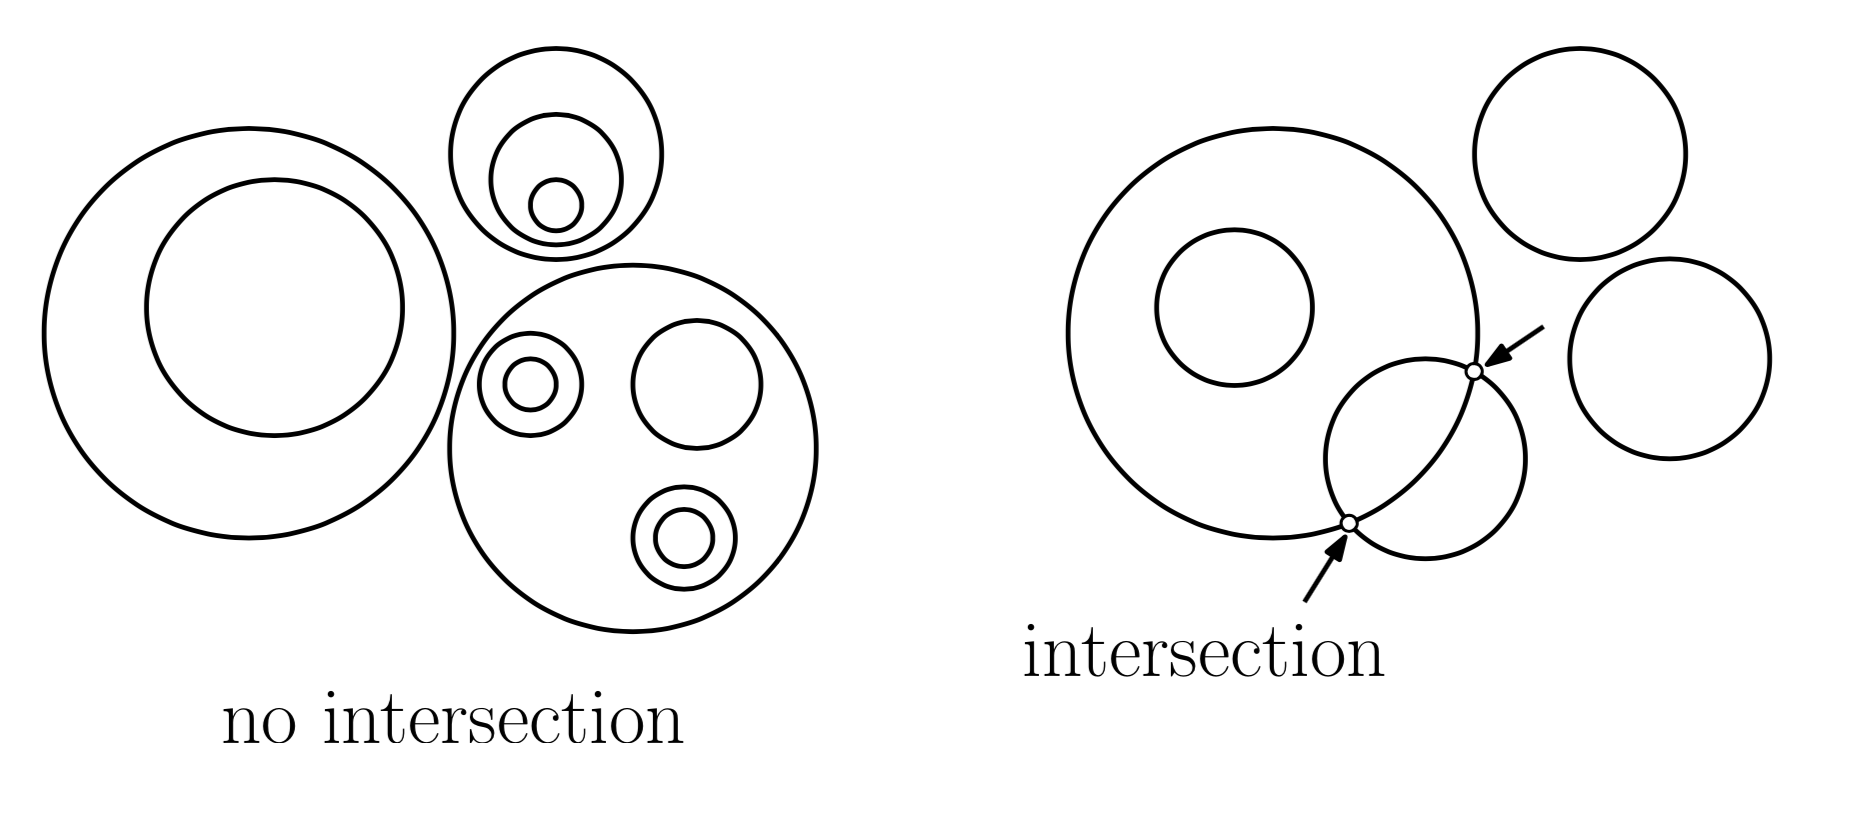
\includegraphics[width=0.75\textwidth]{intersection}
    \caption{Problem 3: Intersection}
\end{figure}

Hint: Use plane-sweep. Explain clearly (1) what the sweep-line status stores and
what data structure is used to store this information and (2) what future events
are stored and what data structure is used. You may assume that you have access
to whatever primitive operations that you need in constant time. For example, if
you want to determine (a) whether two circles intersect, (b) the coordinates of
an intersection, (c) the intersection of a line with a circle, (d) whether a
point is contained within a circle's interior, etc., you may simply assume the
existence of a function that runs in $O(1)$ time. As always, you may make
whatever general-position assumptions you like.

\hrule


So the strategy is to split the circles into two semi circles and treat them individually.
This runs essentially the same as the original line-sweep algorithm for line segments.
The intersection computation is harder since they are not lines, but it can be done in constant time since we have formulas for semi-circles.

\begin{enumerate}[(1)]
    \item The sweepline status stores the semi-circular curves.
        These are stored in a dictionary (balanced tree) and are sorted by the y coordinate (at last event location).
        Ie. The stored y-coordinate is the starting point (left end) of the curve, or the last intersection location.
        Also, a pointer/label of which circle a semi-circle belongs to is stored 
        (this is used to make sure two halves of circle are not considered to intersect, and to return indicies of circles if intersecting)

    \item Our events are the endpoints (left and right) of every circle. 
    Then, at event-time, when a new event occurs, curve intersection is computed between adjacent 
    two semi-circles. If they intersect, a new event is placed at the intersection location. 
    These events are stored in a priority queue. 

    At event-time, the current y-position of adjacent curves is also evaluated. Then neighbors are swapped accordingly.
    This updates the positions of curves so we have current sorted y-levels in the dict. 
\end{enumerate}


\textbf{Runtime and Summary: }So in summary. We add left and right end points to the event queue. 
Then at each event: we update the y value of adjacent semi-circles. 
($O(\log n)$ to find each one, $O(1)$ to evaluate y value, $O(\log n)$ to swap $\implies O(\log n)$)
We then check if intersection: $O(1)$. Then if an intersection is found, we return the two circles.

If the event is a left-endpoint of a circle, we split the circle into two semi circles and add them to the dict.
($O(\log n)$). We also add the upper half semicircle above the lower semicircle in the dict even though both have same initial y coordinate.
If the event is a right end point, we delete the two semi circles ($O(\log n)$)

The algorithm terminates once an intersection is found, so at worst case it takes $O(n \log n)$ time to determine no intersection,
since there are $2n \in O(n)$ events taking $O(\log n)$ time.


\textbf{Correctness: } We show the same lemma as in the straight line segment sweepline algorithm.

\begin{lemma}
    Let $S$ be the set of our circles. Consider $S_i, S_j \in S$ that intersect at $p$.
    Then, $S_i, S_j$ are adjacent on the sweepline prior to event at $p_x$
\end{lemma}

\begin{proof}
    Consider a line $l$ infinitesimally left of $p$. By general position assumptions, 
    no three circles intersect at same point, and no circles intersect at left/right endpoint.
    Thus $S_i, S_j$ are adjacent on sweepline at $l$

    Consider $q$ (event point) with largest $x$ coordinate smaller than $p$.
    Then there are no events between $q$ and $p$. Thus the order on the sweepline does not change between $q$ and $p$.
    Therefore, after processing $q$, $S_i, S_j$ are adjacent on the sweepline.
\end{proof}

Therefore, we only need to check adjacent semi-circles on the sweepline

\problem{4}

I have had a few people ask about drawings and making figures.  One tool that I
like to use is Ipe (written by Otfried Cheong).  Ipe allows you to draw content
on layers and show and hide the different layers.  Layers are very helpful if,
for example you want to draw a point set and then show how some data structures
in an algorithm change as you sweep across the point set.
Other vector graphics tools such asIllustrator and Inkscape are also quite good.

Setup Ipe \url{http://ipe.otfried.org/}, Illustrator, or Inkscape
(or another vector graphics tool)
to create 3 images of the state of the sweep line algorithm
described in problem 3.

\hrule




\end{document}